\chapter*{The description of attached CD}
\label{chap:cd}
\addcontentsline{toc}{chapter}{The description of attached CD}

\begin{figure}[h]
\begin{center}
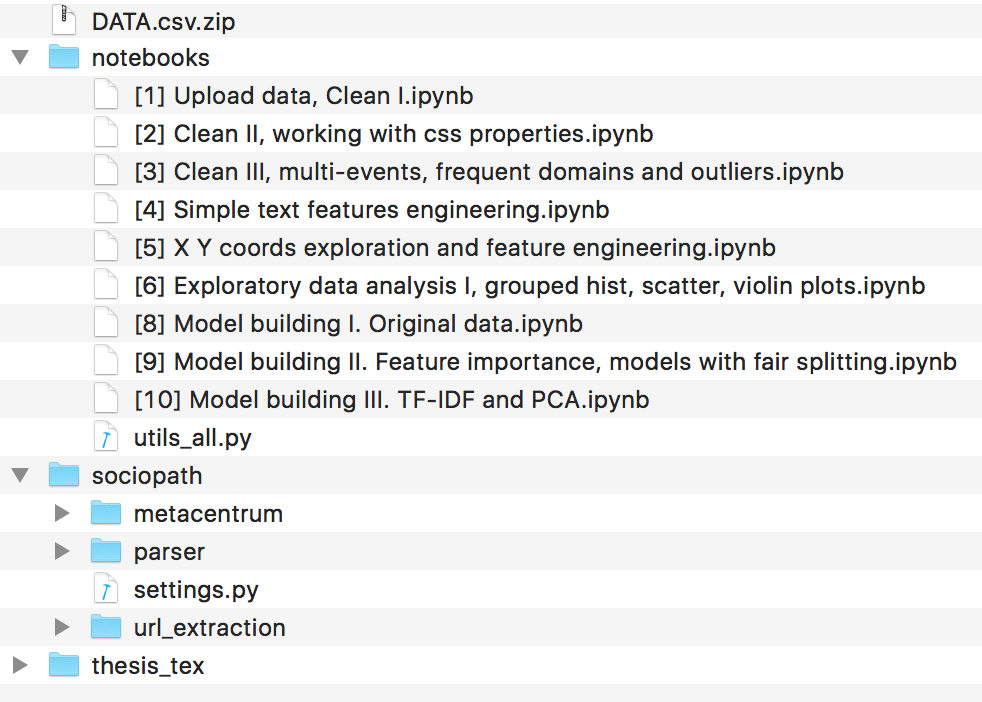
\includegraphics[width=.6\textwidth]{structure}
\caption{Folders structure on attached CD}
\label{fig:cdstructure}
\end{center}
\end{figure}

\begin{itemize}
    \item \textbf{notebooks} - the folder with Jupyter notebooks with analysis and visualizations. Notebooks include some additional images which are not listed in the thesis.
    \item \textbf{sociopath} - the folder with the code of Sociopath parser components
    \item \textbf{thesis\_tex} - $\LaTeX$  project with the thesis text files and images
    \item \textbf{DATA} - published training dataset
\end{itemize}


This project code together with online versions of all notebooks available on GitHub repository: \url{https://github.com/galinaalperovich/Ms-Thesis-CVUT}